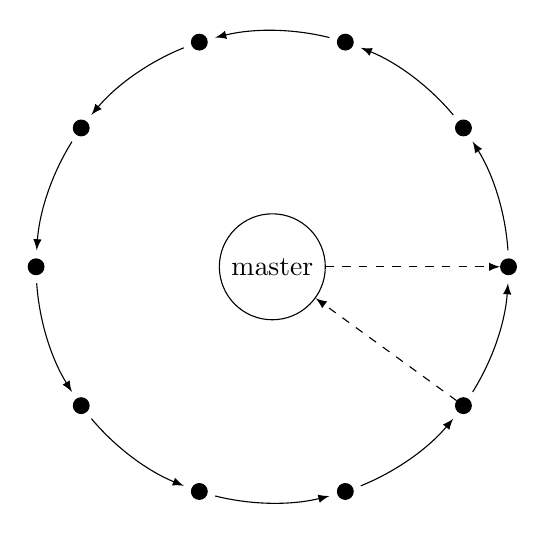
\begin{tikzpicture}
  [place/.style={circle,
    inner sep=0pt,minimum size=2mm}]
  %% from http://www.texample.net/tikz/examples/cycle/
  % Author : Jerome Tremblay
  \def \n {10}
  \def \radius {3cm}
  \def \margin {4} % margin in angles, depends on the radius

  \foreach \s in {1,...,\n}
  {
    \node[draw, circle, fill=black, place] (\s) at ({360/\n * (\s - 1)}:\radius) {};
    \draw[->, >=latex] ({360/\n * (\s - 1)+\margin}:\radius)
    arc ({360/\n * (\s - 1)+\margin}:{360/\n * (\s)-\margin}:\radius);
  }

  \node[draw, circle] (master) at (0:0) {master};
  \draw[->, >=latex, dashed] (master) -- (1);
  \draw[->, >=latex, dashed] (\n) -- (master);
\end{tikzpicture}